\section{Parton Distribution Function} \label{sec:higgs:partons}

The LHC collides protons, however in the Feynman diagrams in
\Cref{fig:higgs_production} it is quarks and gluons (a.k.a partons) that
produce these fundamental interactions. This is an indicator that when the
production cross section is calculated for a process at the LHC, one must not
only consider the hard-scatter probability of the specific diagram, but also
consider the composition of the proton itself.  Furthermore, the calculation
must consider the fraction of the total momentum of the proton held by each of
its constituent partons.  This concept is described by Parton Distribution
Functions (PDFs) which give the probability that the indicated parton carries
momentum fraction $x$ of the proton when probed at energy scale $Q$.  An
example PDF for $Q^2 = 10~\GeV^2$ and $Q^2 = 10^{4}~\GeV^2$ is shown in
\Cref{fig:parton_distribution_function}.

\begin{figure}[!htbp]
  \begin{center}
    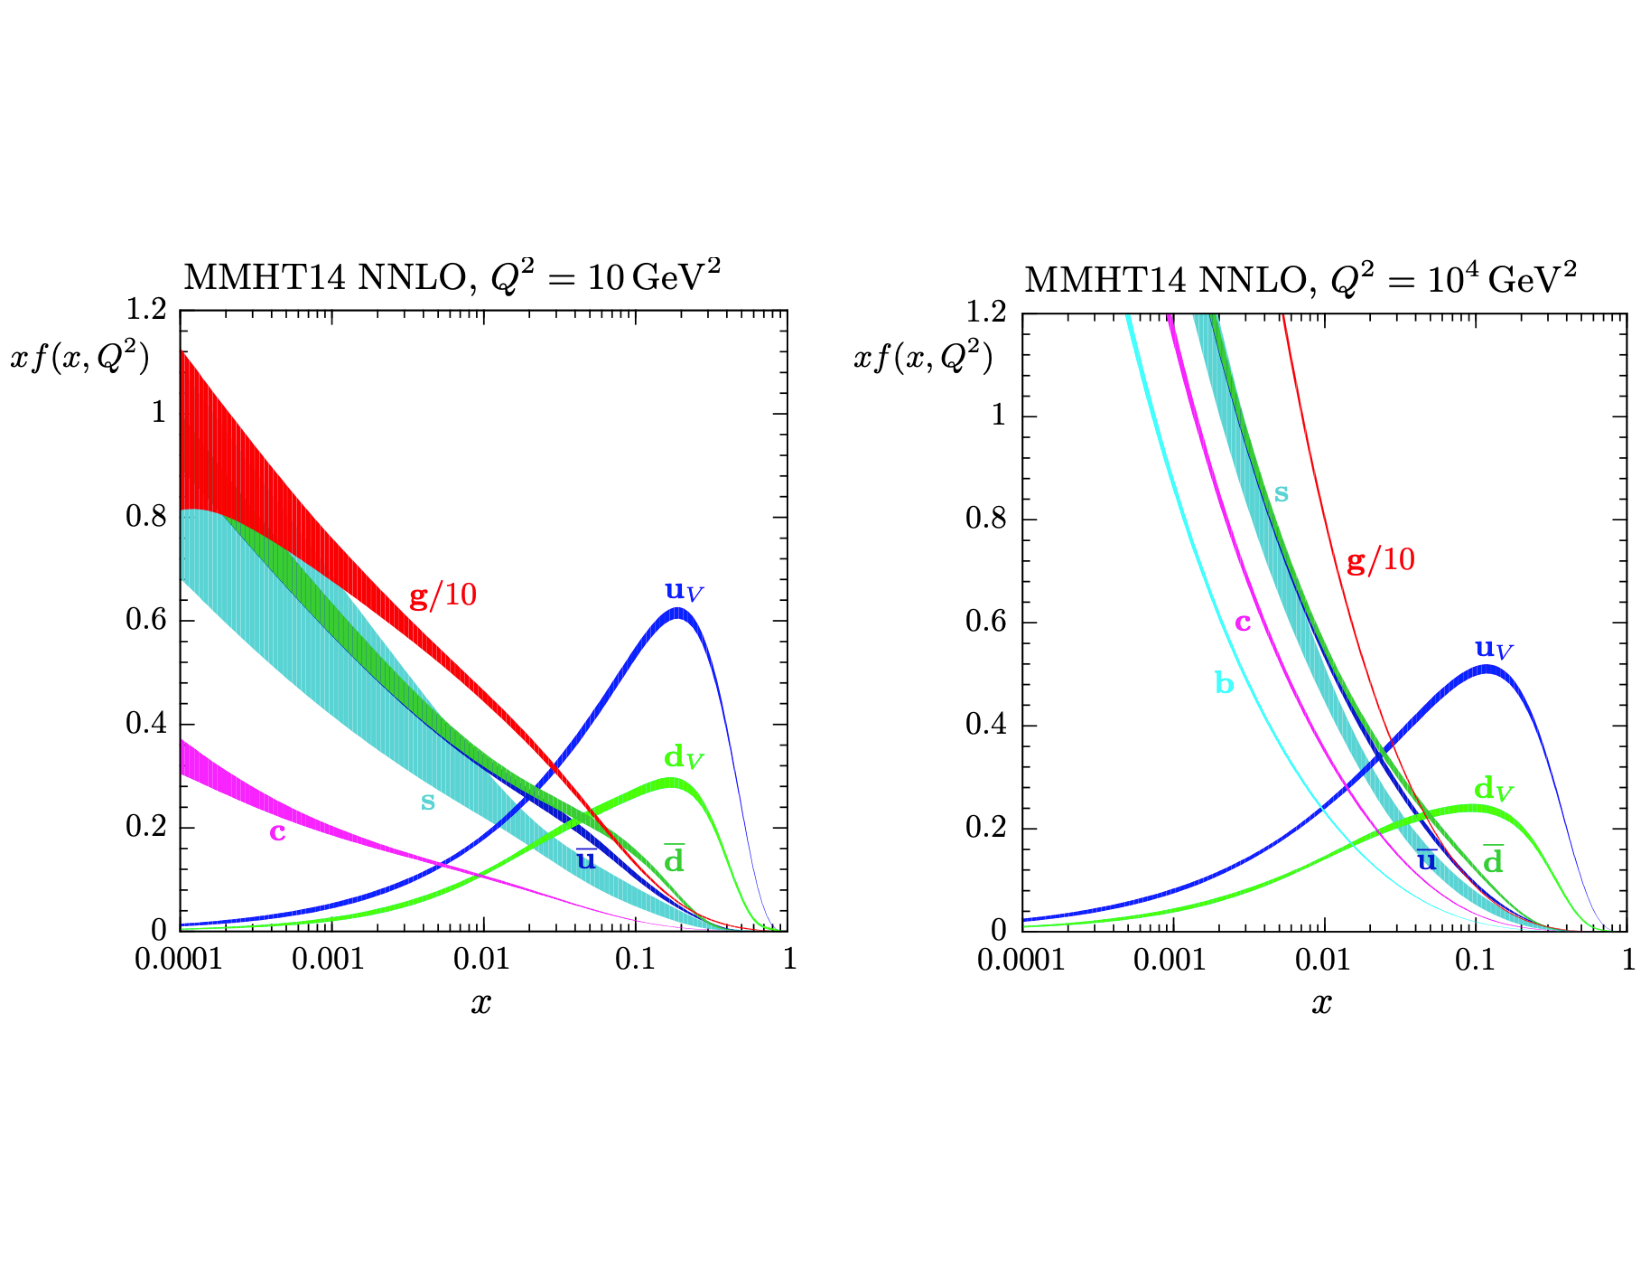
\includegraphics[width=0.8\linewidth]{figures/higgs/pdf.pdf}
    \caption{MMHT2014 NNLO PDFs at $Q^2 = 10~\GeV^{2}$ and $Q^2
=10^{4}~\GeV^{2}$ with associated 68\% confidence-level uncertainty bands
\cite{Harland-Lang2015}.  The colored regions indicate the probability of
finding the labeled parton with a momentum fraction given along the $x$ axis.
As expected the valence quarks contain the largest fraction of the momentum
while the gluons are more likely to carry smaller fractions of the total
momentum.  Note that as $Q^2$ increases the contributions from sea quarks
increases.}
    \label{fig:parton_distribution_function}
  \end{center}
\end{figure}
